\documentclass[12pt]{article}
\usepackage{indentfirst}
%\usepackage{fontspec}
\usepackage[spanish,es-tabla, es-ucroman]{babel}
\usepackage{newtxtext,newtxmath}

\usepackage[utf8]{inputenc}
\usepackage{calc}
\usepackage{pgfplots}
\pgfplotsset{compat=1.18} % o la versión que uses
\usepackage{pgfplotstable}
\usepackage{caption}

\usepackage{float}
\usepackage{caption}
\usepackage{graphicx}
\usepackage{subfigure}
\usepackage{mathtools}
\usepackage{amsmath}
\usepackage{booktabs}
\usepackage{pgfplotstable} 
\usepackage{enumerate} 
\usepackage{amsmath}
\usepackage{graphicx}
\graphicspath{{figuras/}}
\usepackage{parskip}
\usepackage{fancyhdr}
\usepackage{vmargin}
\usepackage{changepage}

\usepackage{multicol}
\usepackage{tikz}
\usepackage{enumitem}
\usetikzlibrary{trees}
\usepackage[table,xcdraw]{xcolor}
\usepackage{array}
\usetikzlibrary{calc}
\setcounter{tocdepth}{2}


% --- Configuración de títulos de tablas/cuadros ---
\usepackage{caption}

\captionsetup[table]{
    font={normalsize},        % base size (lo ajustamos abajo)
    labelfont={normalsize},   % etiqueta "Tabla X"
    textfont={normalsize},    % texto del título
    justification=centering,  % título centrado
    singlelinecheck=false,    % fuerza centrado aunque sea una sola línea
    skip=0pt,                 % sin espacio inferior entre caption y tabla
    position=top              % caption arriba de la tabla
}

% Cambiar tamaño del caption de tablas a 10 pt (Times New Roman)
\makeatletter
\renewcommand\captionfont{\fontsize{10pt}{12pt}\selectfont}
\renewcommand\captionlabelfont{\fontsize{10pt}{12pt}\selectfont}
\makeatother


\usepackage[authoryear,round]{natbib}
% que \cite se comporte como \citep (cita parentética)
\let\oldcite\cite      % por si después querés recuperar el original
\let\cite\citep

\usepackage[pagebackref=true]{hyperref}

\renewcommand*{\backrefalt}[4]{%
  \ifcase #1 (No citado)%
  \or (Citado en la página #2)%
  \else (Citado en las páginas #2)%
  \fi%
}

\setlength{\footskip}{15mm}

% --- Librerías de TikZ que usaremos ---
\usetikzlibrary{
    positioning,  % Para posicionar nodos (below=of, right=of)
    chains,       % Para crear flujos de nodos (A1 -> A2 -> A3...)
    arrows.meta,  % Para flechas bonitas (como 'stealth')
    shapes.misc,  % Para 'rounded rectangle'
    backgrounds   % Para dibujar las cajas de "subgraph" por detrás
}
\usepackage{float} % Para poder usar la opción [H] en las figuras
\usetikzlibrary{positioning, arrows.meta} % Para las flechas y las posiciones

\usetikzlibrary{positioning, arrows.meta, shapes.geometric}

\usepackage[font=small,labelfont=bf,labelsep=period,justification=centering,textfont=it]{caption}



\usepackage{listings}
\usepackage{setspace}
\onehalfspacing

\usepackage{siunitx}
\usepackage{hyperref}
\hypersetup{
    colorlinks=true,
    linkcolor=black,
    citecolor=black,
    urlcolor=black,
    pdfborder={0 0 0}
}

\usepackage{url}
% FUENTE
%setmainfont[BoldFont=arialbd.ttf,
%ItalicFont=ariali.ttf,
%BoldItalicFont=arialbi.ttf]{Arial.ttf}



\definecolor{codebg}{rgb}{0.95,0.95,0.95}
\definecolor{comment}{rgb}{0.15,0.79,0.13}
\definecolor{keyword}{rgb}{0,0,1}
\definecolor{string}{rgb}{0.6,0.1,0.1}

\lstset{
    backgroundcolor=\color{codebg},
    basicstyle=\ttfamily\footnotesize,
    commentstyle=\color{comment},
    keywordstyle=\color{keyword},
    stringstyle=\color{string},
    frame=single,
    breaklines=true,
    showstringspaces=false,
    numbers=left,
    numberstyle=\tiny\color{gray},
    captionpos=b,
    language=Python,
    morekeywords={self}
}

\makeatletter
\renewcommand\footnotesize{\@setfontsize\footnotesize{10pt}{12pt}}
\makeatother


% Estilo BIBLIOFGRAFIA


% CONFIGURACIÓN DE LA HOJA
\setmarginsrb{2.5 cm}{2.5 cm}{2.5 cm}{2.5 cm}{1 cm}{1.5 cm}{1 cm}{0.5 cm}

% CONFIGURACIÓN DE SANGRÍA
\setlength{\parindent}{6mm}
\setlength{\parskip}{1mm}
\setlength{\parskip}{6pt}

%---------------------------------------------------------------------------
%	EN TODAS HOJAS
%---------------------------------------------------------------------------

\title{Actividad 2}				    	% Titulo
\author{Pérez, Matías Agustín}	            % Nombre del estudiante				
\date{30 de Noviembre del 2025}						        % Fecha


\makeatletter
\let\thetitle\@title
\let\theauthor\@author
\let\thedate\@date
\makeatother

%--------------------------------------------------
% ENCABEZADO Y PIE DE PÁGINA PERSONALIZADO
%--------------------------------------------------
\usepackage{lastpage} % para contar el total de páginas
\usepackage{fancyhdr}
\pagestyle{fancy}
\fancyhf{} % limpia encabezado y pie

% ----- ENCABEZADO -----
\lhead{\small\textbf{\thetitle}} % Título arriba a la izquierda
\chead{
\includegraphics[height=1.5cm]{logo_ucasal.jpg}} % Logo centrado
\rhead{\small\textbf{\theauthor}} % Autor arriba a la derecha

% ----- PIE DE PÁGINA -----
\cfoot{\thepage\ de \pageref{LastPage}} % Número de página centrado

% Ajuste de altura para que no se corte el logo
\setlength{\headheight}{28pt}


%%%%%%%%%%%%%%%%%%%%%%%%%%%%%%%%%%%%%%%%%%%%%%%%%%%%%%%%%%%%%%%%%%%%%%%%%%%%%%%%%
%	                                CARÁTULA 
%%%%%%%%%%%%%%%%%%%%%%%%%%%%%%%%%%%%%%%%%%%%%%%%%%%%%%%%%%%%%%%%%%%%%%%%%%%%%%%%%

\pgfplotsset{compat=1.16}
\begin{document}



% CARÁTULA
% CARÁTULA
\begin{titlepage}
\begin{center}
    \vspace*{-3 cm}
    
\includegraphics[scale=0.2]{./figuras/logo_ucasal.jpg}    % logo ucasal
    \vspace{1 cm}

    %%%% TITULO DEL TRABAJO
    \definecolor{Micolor1}{RGB}{130,30,15}                     % color
    \rule{11.9cm}{0.4mm} 

    \Huge \bfseries \textcolor{Micolor1}{Seminario de Tesis}\\[0.7 cm]
 
   
    \textbf{\large \textcolor{Micolor1}{Actividad 2}}
    \vspace{1 cm}

    %%%% NOMBRE DE LA UC
    \textbf {\Large Maestría en Ciencia de Datos}\\[0.3 cm]


    %%%% NOMBRE DE AUTOR Y TUTOR
    \textbf{ \large \textcolor{Micolor1}{Estudiante}}\\ \large{PÉREZ, Matias Agustín}
    \vspace{0.5cm}
    \\
    \textbf{ \large \textcolor{Micolor1}{Director de Tesis}}\\ \large{Dr. ARAUJO, Pedro Bernabé}
    \vspace{0.5cm}
    \\
    \textbf{ \large \textcolor{Micolor1}{Docente de Seminario de Tesis}}\\ \large{Mgtr. NIEVAS, Guillermina Rosana}
    \vspace{0.5 cm}

    % FECHA
    {30 de Noviembre 2025}

    \vfill
\end{center}
\end{titlepage}
%%%%%%%%%%%%%%%%%%%%%%%%%%%%%%%%%%%%%%%%%%%%%%%%%%%%%%%%%%%%%%%%%%%%%%%%%%%%%%%%%
%	                     INICIO DEL DOCUMENTO  
%%%%%%%%%%%%%%%%%%%%%%%%%%%%%%%%%%%%%%%%%%%%%%%%%%%%%%%%%%%%%%%%%%%%%%%%%%%%%%%%%

% %%%%%%% RESUMEN
% \renewcommand{\thepage}{\roman{page}}           %numero de pag romano

% \begin{center}
% \normalsize \textbf{Resumen}
% \end{center}

% \noindent Deberá presentar el objetivo del trabajo, con una breve formulación de la metodología utilizada y las conclusiones o resultados obtenidos. 
% \vspace{0.3cm}

% \noindent \underline{Palabras clave:} Citar tres palabras que representa el estudio.
% \newpage

% %%%%%%% INDICE DE FIGURAS
% \listoffigures
% \addcontentsline{toc}{section}{Índice de figuras}
% \newpage
% \thispagestyle{empty} % quita numero de la pagina

% %%%%%%% ÍNDICE GENERAL
% \tableofcontents
% \newpage
% \pagenumbering{arabic} % cera numero de la pagina

% %%%%%%%%%%%%%% 
% % SECCIÓN 1
% %%%%%%%%%%%%%%



%--------------------------------------------------------------------
% RESUMEN
%--------------------------------------------------------------------

\pagenumbering{arabic} % cera numero de la pagina

% RESUMEN


\section{Planteamiento del Problema}

\subsection{Situación problemática}

Los procesos de acreditación de carreras universitarias ante la \textbf{Comisión Nacional de Evaluación y Acreditación Universitaria (CONEAU)} requieren la recolección, clasificación, vinculación y trazabilidad de una gran cantidad de documentos, evidencias y reportes institucionales \cite{ordenanza62,ordenanza75}. 
Este proceso demanda una elevada carga administrativa y técnica, ya que implica:

\begin{itemize}
    \item analizar criterios y estándares distribuidos en múltiples ordenanzas y documentos normativos;
    \item gestionar cientos de evidencias institucionales con distintos niveles de relevancia y formatos;
    \item coordinar equipos de trabajo, fechas límite y tareas concurrentes;
    \item garantizar la coherencia y trazabilidad del material presentado;
    \item producir informes explicativos y planes de mejora basados en evidencia.
\end{itemize}

Estudios previos muestran que, en universidades argentinas, la fase de autoevaluación suele extenderse más de lo previsto debido a la fragmentación documental, la duplicidad de esfuerzos y la falta de interoperabilidad entre sistemas \cite{sanchez2022acreditacion,duarte2023literature}.  
Asimismo, investigaciones recientes indican que los procesos manuales presentan baja reproducibilidad, escasa estandarización y dificultades para monitorear el avance de criterios complejos \cite{tortosasistemas}.

En paralelo, la aparición de \textbf{Sistemas Multiagente (MAS)}, \textbf{Modelos de Lenguaje (LLM)} y \textbf{protocolos de interoperabilidad como MCP} ha demostrado ser efectiva para coordinar procesos distribuidos, automatizar tareas cognitivas y organizar flujos de trabajo complejos \cite{perez2022breve,sakurada2021multi,farsane2025automatizacion,ehtesham2025survey,agashe2023llm}.  
Sin embargo, su aplicación al dominio específico de la acreditación universitaria en Argentina es prácticamente inexistente, generando un vacío tecnológico y metodológico.

\subsection{Pregunta de investigación}

\textit{¿Cómo puede un sistema multiagente que integre Modelos de Lenguaje (LLM) y un protocolo de interoperabilidad como MCP automatizar y optimizar el seguimiento de los procesos de acreditación de carreras universitarias ante la CONEAU, mejorando la trazabilidad documental, la eficiencia operativa y la consistencia de los informes institucionales?}



\section{Objetivos}

\subsection{Objetivo General}

Formular, diseñar e implementar un \textbf{Sistema Multiagente Inteligente} que integre \textbf{LLM} y \textbf{MCP}, con el propósito de automatizar y optimizar el seguimiento de los procesos de acreditación de carreras universitarias ante la \textbf{CONEAU}, mejorando la trazabilidad, interoperabilidad y eficiencia en la gestión institucional.


\subsection{Objetivos Específicos}

\begin{enumerate}
    \item \textbf{Analizar} el proceso normativo y procedimental de acreditación establecido por la \textbf{CONEAU}, con el fin de identificar las etapas, criterios y flujos de información que puedan ser automatizados mediante un enfoque multiagente.
    
    \item \textbf{Diseñar} la arquitectura general del \textbf{Sistema Multiagente Inteligente}, definiendo los roles, responsabilidades y mecanismos de coordinación entre agentes mediante el \textbf{Model Context Protocol (MCP)}.
    
    \item \textbf{Desarrollar} un agente de \textit{Extracción y Clasificación de Evidencias} que, utilizando técnicas de \textbf{Large Language Models (LLM)}, analice documentos institucionales y asocie evidencias a criterios de acreditación específicos.
    
    \item \textbf{Implementar} un agente de \textit{Evaluación de Cumplimiento} que determine el nivel de cumplimiento de los estándares definidos por la CONEAU, justificando sus conclusiones mediante razonamiento explicable.
    
    \item \textbf{Diseñar} un agente de \textit{Seguimiento Continuo} que supervise las tareas de la comisión de autoevaluación, detecte retrasos y emita alertas automáticas para optimizar la gestión de tiempos.
    
    \item \textbf{Integrar} los módulos desarrollados en un \textit{dashboard interactivo} que visualice el estado general del proceso de acreditación, el avance por estándar y los indicadores clave de desempeño institucional.
    
    \item \textbf{Documentar} la arquitectura y el funcionamiento del sistema, proponiendo recomendaciones para su futura extensión con módulos de \textit{Recomendaciones y Planes de Mejora} basados en análisis de brechas detectadas.
\end{enumerate}

\section*{Estado del Arte}

El presente estado del arte revisa críticamente tres cuerpos de conocimiento relevantes para el desarrollo del sistema propuesto:  
\begin{enumerate}
    \item Los marcos normativos y procedimentales de la acreditación universitaria argentina;  
\item Los avances en Sistemas Multiagente (MAS), inteligencia distribuida y coordinación cognitiva; y  
\item Las aplicaciones recientes de modelos de lenguaje (LLM), automatización documental y protocolos de interoperabilidad como MCP.  
\end{enumerate}


El objetivo es identificar los aportes existentes, sus limitaciones y el vacío técnico–metodológico que justifica el desarrollo de este trabajo.

\subsection{Acreditación universitaria: normativa, debilidades y desafíos}

Los procesos de acreditación de carreras de ingeniería en Argentina se encuentran regulados por las normativas emitidas por la \textbf{CONEAU}, particularmente la Ordenanza N° 62/2017 \cite{ordenanza62} y sus normas complementarias, entre ellas la Ordenanza N° 75/2023 \cite{ordenanza75}.  
Estas regulaciones establecen criterios, estándares, evidencias mínimas y procedimientos que deben cumplirse durante la autoevaluación y evaluación externa.

Si bien los documentos normativos definen con claridad los criterios de calidad, no especifican mecanismos tecnológicos para gestionar la creciente complejidad documental. Por ello, instituciones y comisiones de autoevaluación enfrentan desafíos importantes:

\begin{itemize}
    \item \textbf{Fragmentación y heterogeneidad documental:} los insumos provienen de múltiples fuentes (departamentos, áreas administrativas, sistemas locales).
    \item \textbf{Falta de trazabilidad:} los documentos no suelen mantener un historial de versiones ni un registro claro de su vinculación con cada estándar.
    \item \textbf{Altos costos temporales y cognitivos:} la lectura, clasificación y vinculación manual de evidencias demanda cientos de horas de trabajo académico.
    \item \textbf{Baja reproducibilidad:} equipos diferentes clasifican y redactan informes de forma no homogénea.
\end{itemize}

La literatura especializada en acreditación latinoamericana coincide en estas limitaciones.  
Duarte \cite{duarte2023literature} identifica que los sistemas de acreditación presentan cuellos de botella en: trazabilidad, heterogeneidad de formatos, repetición de tareas y ausencia de herramientas de apoyo inteligente.  
Asimismo, documentos del CONFEDI \cite{sanchez2022acreditacion} señalan que las instituciones dependen fuertemente de esfuerzos manuales y no logran consolidar mecanismos estandarizados de seguimiento.

En síntesis, las fuentes normativas describen \textbf{qué} se debe evaluar, pero no \textbf{cómo} gestionar técnicamente el flujo de documentos, lo cual crea un espacio para soluciones basadas en inteligencia artificial e interoperabilidad.

\subsection{Sistemas Multiagente y coordinación distribuida}

Los \textbf{Sistemas Multiagente (MAS)} han demostrado ser eficaces para organizar tareas complejas en dominios donde intervienen múltiples actores, documentos y reglas.  
Pérez \cite{perez2022breve} realiza un repaso exhaustivo de las metodologías MAS y destaca que su aporte principal consiste en la descomposición funcional del problema en agentes autónomos y cooperativos. El autor enfatiza tres ventajas relevantes:

\begin{itemize}
    \item distribución funcional del problema en tareas especializadas;
    \item comunicación explícita entre agentes mediante protocolos formales;
    \item capacidad de adaptación frente a entornos dinámicos.
\end{itemize}

Por su parte, Sakurada \cite{sakurada2021multi} muestra que los MAS pueden operar como \textbf{capas de organización inteligente} en sistemas industriales complejos, extendiendo su aplicabilidad a procesos que requieren trazabilidad, monitoreo y razonamiento distribuido.  
Un punto crítico de este trabajo es que resalta la importancia del “\textit{asset administration shell}”, un concepto que se asemeja a la necesidad de mantener metadatos, versiones y relaciones de evidencias, tal como ocurre en los procesos de acreditación.

La literatura revisada coincide en que los MAS son idóneos para:

\begin{itemize}
    \item coordinar tareas asincrónicas;
    \item integrar fuentes de información heterogéneas;
    \item escalar procesos que requieren múltiples actores simultáneos;
    \item sostener flujos de trabajo basados en roles.
\end{itemize}

Sin embargo, no existen antecedentes de MAS aplicados al aseguramiento de la calidad universitaria en Argentina.

\subsection{IA generativa, automatización documental y análisis semántico}

Diversos trabajos recientes muestran el potencial de combinar IA con procesos documentales complejos.

Tortosa \cite{tortosasistemas} presenta sistemas inteligentes para el seguimiento de proyectos ágiles, destacando que los modelos de IA pueden:

\begin{itemize}
    \item extraer información relevante,
    \item clasificar documentos,
    \item identificar riesgos y brechas,
    \item sugerir acciones de mejora.
\end{itemize}

Cascavita \cite{cascavita2025sistema} y Farsane \cite{farsane2025automatizacion} demuestran que agentes inteligentes y pipelines de IA pueden automatizar flujos documentales de gran volumen, incorporando técnicas de OCR, análisis semántico y workflows.  
Estas investigaciones aportan evidencia empírica de que los sistemas inteligentes mejoran:

\begin{itemize}
    \item la calidad del registro documental,
    \item la velocidad de procesamiento,
    \item la consistencia en la clasificación,
    \item la generación automática de informes.
\end{itemize}

Aunque sus contextos no son educativos, los paralelismos con la acreditación universitaria son evidentes: grandes volúmenes de documentos, necesidad de clasificación, trazabilidad y generación de reportes explicativos.

Agashe \cite{agashe2023llm} introduce explícitamente la integración de \textbf{LLM en sistemas multiagente}, demostrando que los modelos de lenguaje pueden cumplir roles complejos como:

\begin{itemize}
    \item agentes de razonamiento,
    \item mediadores de decisiones,
    \item generadores de explicaciones,
    \item clasificadores semánticos.
\end{itemize}

Este es un aporte crucial, pues valida que los LLM pueden incorporarse a MAS como componentes cognitivos dentro de flujos reales de trabajo.

\subsection{Interoperabilidad y protocolos emergentes: el rol de MCP}

El \textbf{Model Context Protocol (MCP)} es presentado por Ehtesham \cite{ehtesham2025survey} como un protocolo emergente para la coordinación de agentes, recursos y modelos de IA.  
Su relevancia radica en tres aspectos que coinciden directamente con las necesidades institucionales de acreditación:

\begin{itemize}
    \item comunicación estandarizada entre agentes heterogéneos;
    \item trazabilidad completa mediante intercambio de mensajes estructurados;
    \item integración de recursos distribuidos (archivos, bases de datos, servicios externos).
\end{itemize}

Mientras que las ordenanzas CONEAU no especifican mecanismos técnicos para la gestión integral de evidencias, MCP ofrece una capa de interoperabilidad basada en estándares que permite auditabilidad y control, algo sumamente valioso para instituciones que deben demostrar cumplimiento normativo.

No se identifican aplicaciones de MCP en educación superior, lo que confirma la originalidad del enfoque propuesto.

\subsection{Síntesis crítica y vacío identificado}

De la revisión realizada puede afirmarse que:

\begin{itemize}
    \item Los procesos de acreditación son complejos, manuales y altamente dependientes de gestión documental \cite{ordenanza62,duarte2023literature}.
    \item Existen avances sólidos en MAS y coordinación distribuida \cite{perez2022breve,sakurada2021multi}.
    \item La IA generativa permite automatizar clasificación, análisis y redacción \cite{tortosasistemas,cascavita2025sistema,agashe2023llm}.
    \item MCP habilita interoperabilidad y trazabilidad \cite{ehtesham2025survey}.
\end{itemize}

Sin embargo, \textbf{no existe ninguna propuesta que combine estas tres dimensiones (MAS + LLM + MCP) aplicada específicamente a la acreditación universitaria regulada por CONEAU}.  
La literatura tampoco ofrece soluciones de:

\begin{itemize}
    \item seguimiento automatizado por estándar;
    \item clasificación semántica de evidencias normativas;
    \item generación automática de reportes para autoevaluación o planes de mejora;
    \item monitoreo de plazos y responsabilidades institucionales;
    \item trazabilidad auditable de documentos mediante protocolos formales.
\end{itemize}

Este vacío constituye una oportunidad clara para el desarrollo de un sistema multiagente inteligente que aborde la complejidad normativa, operativa y documental de los procesos de acreditación en Argentina.


\section{Breve Marco Teórico Inicial}

\subsection{Contexto normativo y procesos de acreditación en Argentina}

El sistema de aseguramiento de la calidad en la educación superior argentina se estructura en torno a la \textbf{Comisión Nacional de Evaluación y Acreditación Universitaria (CONEAU)}, organismo descentralizado creado por la Ley de Educación Superior N° 24.521, con el mandato de evaluar y acreditar las carreras universitarias, especialmente aquellas incluidas en el artículo 43 de dicha ley, por su impacto en el interés público.

La CONEAU establece procedimientos específicos para las distintas etapas de evaluación mediante ordenanzas. En particular:
\begin{itemize}
    \item La \textbf{Ordenanza N° 62/17} define el procedimiento para la evaluación de proyectos de carreras de grado o carreras nuevas, orientado al reconocimiento oficial provisorio de títulos.
    \item La \textbf{Ordenanza N° 75/23} regula la acreditación de carreras de grado en funcionamiento, mediante procesos de autoevaluación, evaluación externa por pares y dictamen final \cite{ordenanza62, ordenanza75}.
\end{itemize}

Ambos procedimientos demandan una importante carga administrativa y documental, con múltiples actores involucrados: equipos de autoevaluación institucional, comités de pares, comisiones de área y el propio plenario de la CONEAU. Este ecosistema organizacional genera un entorno complejo, con alto volumen de información, plazos estrictos y múltiples versiones de documentos. La literatura en gestión de calidad educativa (Sánchez, 2022; Duarte, 2023) coincide en que esta complejidad representa uno de los principales desafíos para la trazabilidad y transparencia de los procesos \cite{sanchez2022acreditacion, duarte2023literature}.

A continuación, la Figura~\ref{fig:procesos_coneau} sintetiza de manera comparativa los flujos normativos definidos por la CONEAU para carreras nuevas y carreras en funcionamiento, según sus respectivas ordenanzas.



\begin{figure}[H]
\centering
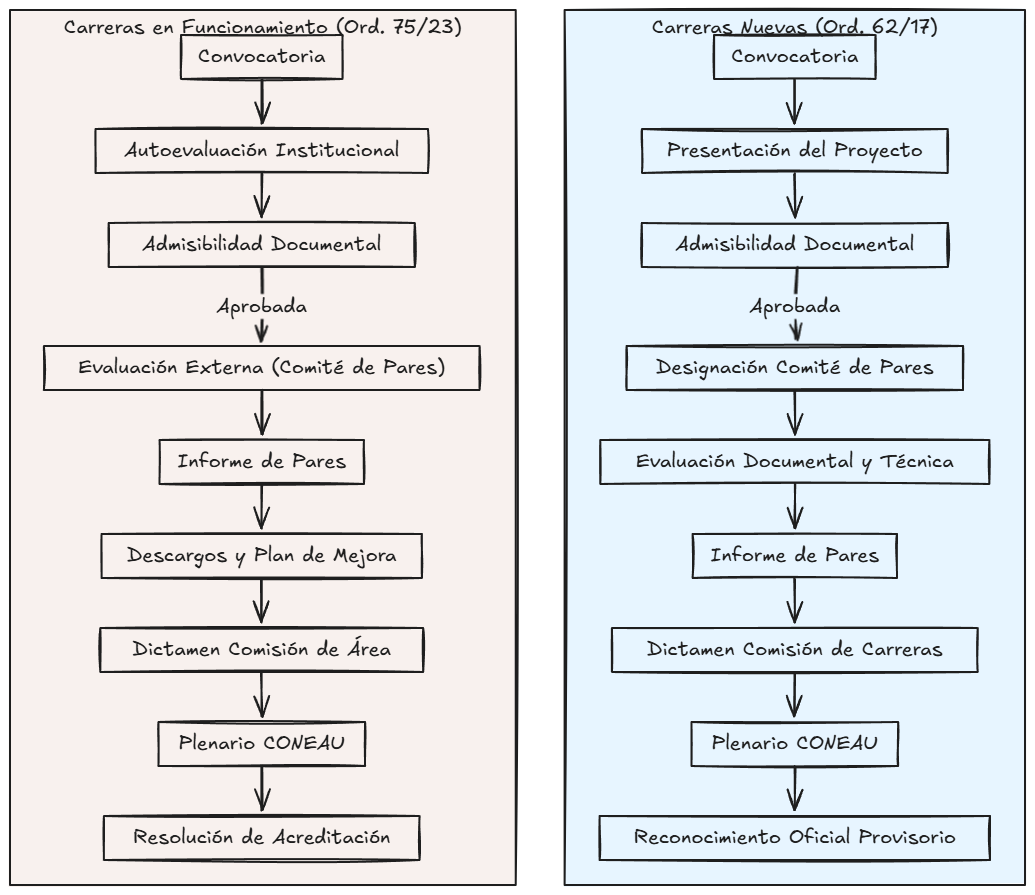
\includegraphics[width=0.85\linewidth]{procedimientonuevoyfuncioando.png}
\caption{Comparación de los procesos de acreditación establecidos por CONEAU para carreras nuevas y carreras en funcionamiento. \textbf{Fuente:} Elaboración propia en base a las Ordenanzas N° 62/17 y N° 75/23.}
\label{fig:procesos_coneau}
\end{figure}

En ambos casos, los procesos presentan una estructura secuencial con ciclos de revisión y validación cruzada, donde cada instancia depende de la resolución de la anterior. Esta dinámica, aunque garantiza el control de calidad, suele generar redundancia documental y dilaciones temporales, lo cual justifica la necesidad de herramientas inteligentes que automaticen la gestión y el seguimiento de estas etapas.

Desde una perspectiva institucional, la implementación de mecanismos digitales de trazabilidad se ha convertido en un requisito clave para optimizar la gestión universitaria y responder a las demandas de mejora continua planteadas por la propia CONEAU y los lineamientos del CONFEDI. En los últimos años, diversas investigaciones han señalado que la automatización y el uso de tecnologías inteligentes permiten mejorar la coherencia de los procesos de acreditación y fortalecer la cultura de calidad institucional \cite{farsane2025automatizacion, duarte2023literature}.




\subsection{Enfoques teóricos de los Sistemas Multiagente (MAS)}

Los \textbf{Sistemas Multiagente} (\textbf{MAS}, por sus siglas en inglés) constituyen uno de los paradigmas centrales dentro del campo de la \textbf{Inteligencia Artificial Distribuida}. Un MAS está conformado por un conjunto de agentes autónomos que interactúan entre sí en un entorno compartido, cooperando para alcanzar un objetivo común mediante la coordinación de sus acciones individuales \cite{perez2022breve}. 

De acuerdo con \cite{sakurada2021multi}, los sistemas multiagente ofrecen una base conceptual sólida para representar y gestionar la complejidad de entornos dinámicos, distribuyendo la inteligencia entre entidades especializadas. Este enfoque resulta particularmente adecuado para contextos donde participan múltiples actores, se aplican reglas diferenciadas y existen dependencias temporales entre tareas, como ocurre en los procesos administrativos y académicos de las instituciones universitarias.

En el marco de esta investigación, los agentes que conforman el sistema pueden asumir diferentes roles funcionales, definidos a partir de sus responsabilidades y del tipo de información que gestionan:
\begin{itemize}
    \item \textbf{Agente Coordinador:} organiza las tareas, distribuye los objetivos entre los demás agentes y gestiona la resolución de conflictos.
    \item \textbf{Agente Documental:} administra la clasificación, almacenamiento y vinculación de evidencias y anexos normativos asociados al proceso de acreditación.
    \item \textbf{Agente de Comunicación (LLM):} procesa información textual, genera resúmenes, interpreta consultas en lenguaje natural y asiste en la elaboración de informes técnicos.
    \item \textbf{Agente de Interoperabilidad (MCP):} gestiona el intercambio de datos y garantiza la comunicación segura entre el sistema multiagente y las plataformas institucionales externas.
\end{itemize}

Esta estructura modular y distribuida coincide con las características definidas por \cite{perez2022breve}, quienes destacan la capacidad de los MAS para modelar entornos organizacionales complejos mediante agentes autónomos, cooperativos y comunicativos. De manera complementaria, \cite{farsane2025automatizacion} subraya que la incorporación de agentes inteligentes en flujos de trabajo administrativos contribuye significativamente a mejorar la trazabilidad, la coherencia y la eficiencia de los procesos.

El funcionamiento de un MAS se fundamenta en la interacción de múltiples entidades autónomas —denominadas \textit{agentes}— que colaboran de forma coordinada dentro de un entorno compartido. En la \textbf{Figura~\ref{fig:mas_estructural}} se presenta de manera conceptual la estructura general de un sistema multiagente, en la que cada agente desempeña un rol específico pero interdependiente.

\begin{itemize}
    \item El \textbf{Agente Coordinador} actúa como núcleo organizativo, planificando las acciones y distribuyendo las tareas entre los distintos agentes.
    \item El \textbf{Agente de Procesamiento} ejecuta operaciones analíticas o de cálculo, constituyendo el componente operativo del sistema.
    \item El \textbf{Agente de Comunicación} mantiene el vínculo con los usuarios o sistemas externos, transformando los datos técnicos en información comprensible.
    \item El \textbf{Agente de Monitoreo} supervisa el estado general del sistema, detecta anomalías o demoras y retroalimenta al coordinador para optimizar el comportamiento del conjunto.
\end{itemize}

El \textbf{entorno de interacción} comprende tanto a los usuarios institucionales como a las fuentes de datos, repositorios documentales y sistemas externos con los que los agentes intercambian información. Este diseño agnóstico permite adaptar la arquitectura multiagente a distintos contextos de aplicación —desde la gestión universitaria hasta ámbitos industriales o empresariales— sin modificar los principios esenciales de autonomía, cooperación y coordinación que caracterizan a este enfoque.

\begin{figure}[H]
\centering
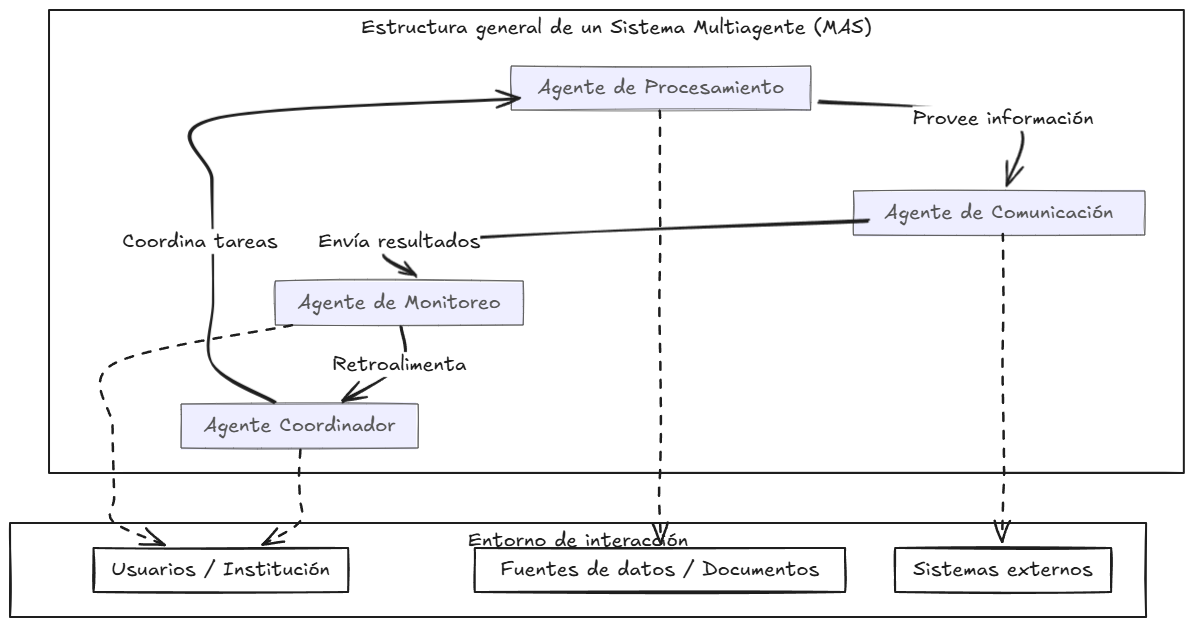
\includegraphics[width=0.85\linewidth]{estructurageneraldeunMAS.png}
\caption{Estructura general de un Sistema Multiagente (MAS). \textbf{Fuente}: Elaboración propia.}
\label{fig:mas_estructural}
\end{figure}


\subsection{Large Language Models (LLM)}

Los \textbf{Large Language Models (LLM)} representan una de las innovaciones más significativas en el campo de la inteligencia artificial contemporánea. Basados en arquitecturas de redes neuronales profundas, como los \textit{transformers\footnote{Arquitectura de modelos de aprendizaje profundo basada en mecanismos de atención, utilizada principalmente en procesamiento de lenguaje natural y visión por computadora.}
}, los LLM son capaces de procesar y generar lenguaje natural a partir de la identificación de patrones estadísticos en grandes volúmenes de texto. Su capacidad para comprender el contexto semántico y producir respuestas coherentes los convierte en una herramienta de gran valor para tareas que requieren interpretación, síntesis y razonamiento lingüístico \cite{agashe2023llm}.

Según Agashe, la evolución de los LLM ha permitido desarrollar agentes capaces de coordinarse entre sí mediante el intercambio de mensajes en lenguaje natural, reduciendo la necesidad de programación explícita y potenciando la adaptabilidad del sistema. Esta característica los posiciona como un componente fundamental en la nueva generación de \textbf{sistemas multiagente cognitivos}, donde cada agente puede incorporar un modelo lingüístico como núcleo de razonamiento contextual.

En el ámbito de la educación superior y la gestión institucional, los LLM presentan un potencial considerable para asistir en tareas de análisis documental, extracción de información, clasificación semántica y generación de reportes automatizados. Aplicados al contexto de la acreditación de carreras universitarias, estos modelos pueden procesar informes de autoevaluación, dictámenes de pares evaluadores o planes de mejora, generando resúmenes estructurados y detectando relaciones entre evidencias y estándares de calidad definidos por la CONEAU.

En el marco de esta investigación, los LLM se conciben como \textbf{agentes semánticos} dentro del Sistema Multiagente propuesto, dotados de capacidades de comprensión y generación de lenguaje natural. Estos agentes pueden:
\begin{itemize}
    \item Interpretar consultas en lenguaje natural provenientes de usuarios institucionales o del Agente Coordinador.
    \item Analizar documentos textuales y extraer información relevante para su clasificación en criterios de acreditación.
    \item Generar reportes o recomendaciones automáticas en función de los hallazgos, manteniendo coherencia terminológica con la normativa vigente.
    \item Colaborar con otros agentes del sistema, utilizando el lenguaje como medio de coordinación contextual.
\end{itemize}

Como se ilustra en la \textbf{Figura~\ref{fig:llm_contextual}}, los LLM pueden integrarse dentro del sistema multiagente como módulos autónomos de procesamiento semántico, interactuando con agentes funcionales y el entorno de información institucional. Esta integración amplía las capacidades del sistema al combinar la \textit{autonomía de los agentes} con la \textit{inteligencia contextual de los modelos de lenguaje}, generando así un marco de interacción explicable y adaptable.

\begin{figure}[H]
    \centering
    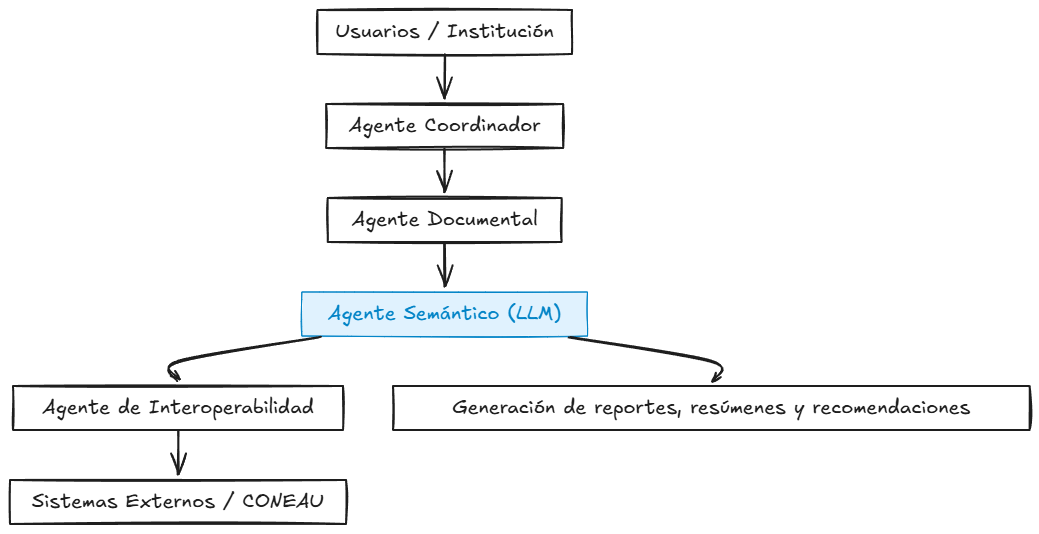
\includegraphics[width=0.75\linewidth]{integracionllm.png}

\caption{Integración de un LLM como agente semántico dentro del Sistema Multiagente. \textbf{Fuente}: Elaboración propia.}
\label{fig:llm_contextual}
\end{figure}

Diversos estudios confirman la pertinencia de esta integración. \cite{farsane2025automatizacion} destaca que la incorporación de modelos de lenguaje en sistemas inteligentes de gestión permite mejorar la calidad del análisis documental, reducir la carga operativa y aumentar la coherencia textual entre diferentes fuentes institucionales. Asimismo, esta tendencia se enmarca en el movimiento hacia una \textbf{IA explicable y colaborativa}, donde los sistemas no solo automatizan procesos, sino que también comunican su razonamiento de manera transparente.


\subsection{Model Context Protocol (MCP)}

El \textbf{Model Context Protocol (MCP)} es un estándar emergente que define un conjunto de reglas e interfaces para posibilitar la comunicación estructurada entre modelos de lenguaje, agentes inteligentes y sistemas externos. Propuesto en el marco de la interoperabilidad de la inteligencia artificial generativa, el MCP proporciona un lenguaje común para el intercambio de contexto, datos y tareas entre componentes autónomos \cite{ehtesham2025survey}.

De acuerdo con Ehtesham, el MCP se basa en un modelo de mensajería bidireccional estructurado en \textit{JSON-RPC}, lo que permite que distintos agentes o modelos compartan información semántica de manera segura, verificable y trazable. Esta estructura reduce la dependencia de integraciones ad hoc y facilita la coordinación de flujos de trabajo en sistemas distribuidos, en los cuales cada agente puede ejecutar funciones especializadas sin perder coherencia global.

La \textbf{Figura~\ref{fig:mcp_interoperabilidad}} muestra un esquema conceptual de cómo el MCP actúa como capa de interoperabilidad dentro del Sistema Multiagente propuesto. En este modelo, el protocolo establece canales de comunicación estandarizados que permiten a los agentes intercambiar mensajes y contexto operativo, garantizando la consistencia y trazabilidad de la información.

\begin{figure}[H]
\centering

    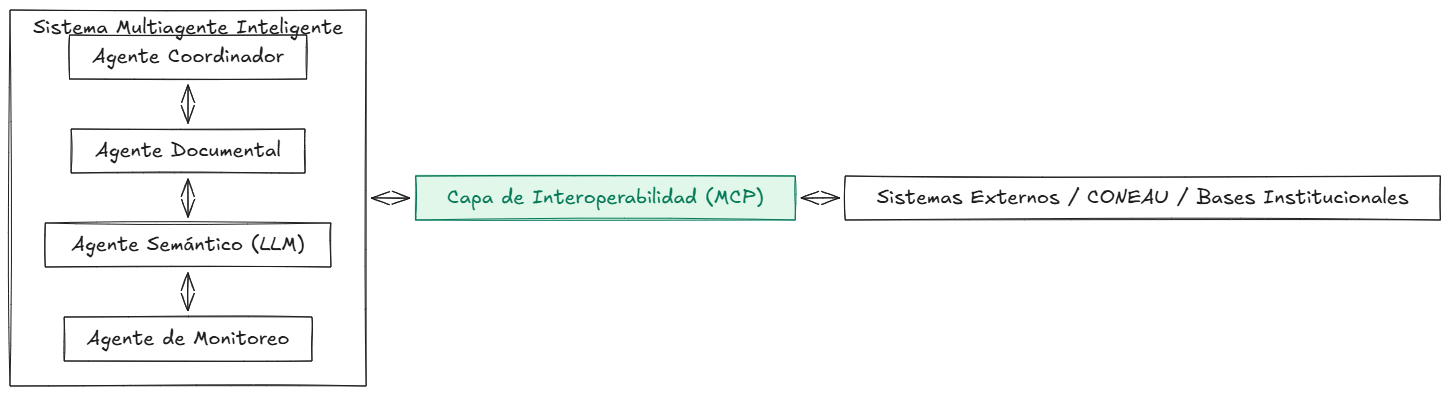
\includegraphics[width=0.85\linewidth]{interoperabilidad.png}

\caption{El MCP como capa de interoperabilidad en la arquitectura multiagente. \textbf{Fuente}: Elaboración propia.}
\label{fig:mcp_interoperabilidad}
\end{figure}

El rol del MCP en esta investigación es habilitar la \textbf{interoperabilidad semántica y funcional} entre los agentes del sistema multiagente y los sistemas institucionales utilizados durante los procesos de acreditación. A través de este protocolo, cada agente puede intercambiar información sobre el estado de las tareas, los documentos procesados o los resultados analíticos, utilizando un formato unificado y fácilmente interpretable.

En términos prácticos, el MCP actúa como una \textit{capa de comunicación contextual} que:
\begin{itemize}
    \item Permite que los agentes compartan información en un formato estructurado y estandarizado.
    \item Garantiza la trazabilidad de los mensajes intercambiados entre módulos o componentes.
    \item Facilita la integración del sistema con herramientas externas (bases de datos, repositorios documentales, plataformas institucionales, etc.).
    \item Soporta la ejecución coordinada de tareas complejas mediante el intercambio de contexto operativo.
\end{itemize}

Esta capacidad de comunicación estructurada constituye un avance significativo respecto de los enfoques tradicionales de integración, en los que los agentes dependían de canales de comunicación rígidos o específicos de cada aplicación. Como señala Farsane, la adopción de protocolos de interoperabilidad y trazabilidad permite que los sistemas inteligentes se integren más fácilmente con entornos organizacionales complejos, aportando transparencia y eficiencia a los procesos administrativos y decisionales \cite{farsane2025automatizacion}.

De este modo, la incorporación del \textbf{Model Context Protocol (MCP)} en el sistema multiagente propuesto no solo facilita la conexión entre agentes y modelos de lenguaje, sino que también sienta las bases para un ecosistema inteligente institucional interoperable, donde las decisiones y los flujos de información pueden ser auditados, replicados y comprendidos de manera explicable.


\subsection{Articulación conceptual del Sistema Multiagente propuesto}


La integración de estos tres enfoques (MAS, LLM y MCP) responde a la necesidad de gestionar entornos institucionales complejos, caracterizados por grandes volúmenes de información, múltiples actores y procesos normativos rigurosos. En este sentido, el \textbf{MAS} proporciona la estructura organizacional distribuida que permite representar los diferentes actores institucionales y sus interacciones. Cada agente actúa como una unidad autónoma que ejecuta tareas específicas, comunicándose mediante protocolos estandarizados y cooperando para alcanzar los objetivos comunes del sistema.

Los \textbf{LLM} amplían las capacidades cognitivas de los agentes, dotándolos de comprensión semántica, razonamiento contextual y generación de texto coherente. Estos agentes semánticos son capaces de analizar documentos complejos —como informes de autoevaluación, dictámenes o resoluciones—, identificar evidencias y producir reportes o recomendaciones en lenguaje natural, facilitando la comunicación entre los usuarios institucionales y el sistema \cite{agashe2023llm,farsane2025automatizacion}.

Por su parte, el \textbf{MCP} actúa como una capa transversal de interoperabilidad que permite el intercambio seguro y estructurado de información entre los agentes del sistema y las plataformas institucionales externas. Esta capa de comunicación basada en contexto asegura la trazabilidad de los datos, la transparencia de las operaciones y la escalabilidad del sistema en distintos entornos organizacionales \cite{ehtesham2025survey}.


Esta articulación permite concebir un ecosistema inteligente orientado a la \textbf{automatización, trazabilidad e interoperabilidad} de los procesos de acreditación. El sistema resultante puede supervisar el flujo documental, clasificar evidencias, generar reportes explicativos y mantener comunicación continua con los actores institucionales, todo ello dentro de un marco de transparencia y eficiencia alineado con los lineamientos de la CONEAU.

Asimismo, el enfoque propuesto se alinea con las tendencias internacionales de \textbf{IA colaborativa y explicable}, donde los sistemas no solo ejecutan tareas automáticas, sino que también son capaces de justificar sus resultados y adaptarse a nuevas condiciones del entorno. Este principio es esencial para garantizar la confiabilidad del sistema dentro de un contexto regulado como el de la educación superior.




\bibliographystyle{apalike}
\bibliography{referencias}








\end{document}
